\section{Model}

The TMD system is described by
the effective tight-biding, low-energy, two-valley Hamiltonian
\cite{PhysRevLett.108.196802},
\begin{equation}
  \label{eq:hamiltonian}
  H_τ^0 \ofK
  = a t \left( τ k_x \hat{σ}_x + k_y \hat{σ}_y \right)
  + \frac{E_g}{2} \hat{σ}_z - E_{\text{soc}} τ \frac{\hat{σ}_z - 1}{2} \hat{s}_z.
\end{equation}
where the Pauli matrices $\hat{s}_i$ operate in the spin space and
$\hat{σ}_i$ operate in the orbital space
with the two Bloch orbital states $\ketOrb{ν}{\ofK}$
(indexed by $ν = +$ for the in-plane orbital state
$\Ket{d_{x^2 - y^2}} + i τ \Ket{d_{xy}}$
and $ν = -$ for the out-of-plane orbital state $\Ket{d_{z^2}}$),
${\s} = ±$ is the spin index, and $τ = ±$ is the valley index corresponding
to the $± \vc{K}$ point, respectively.
The momentum $\vK = \left( k_x, k_y \right)$
is measured from the valley center, $a$ is the lattice constant,
$t$ is the hopping parameter, $E_g$ represents the energy
gap between the conduction and valence bands, and $2E_{\text{soc}}$ is the
spin splitting energy in the valence bands due to spin-orbit interaction.

The energy spectrum,
\begin{equation}
  \label{eq:energy}
  2 \fnEnergy{n} \of{k}
  = τ {\s} E_{\text{soc}} + n \sqrt{{\left( 2 a t k \right)}^2
  + {\left( E_g - τ {\s} E_{\text{soc}} \right)}^2}.
\end{equation}
with $k = \abs{\vK}$
and $n = 1$ ($n = -1$) indexing the conduction (valence) band
is shown in \cref{fig:energy}.

\begin{figure}
  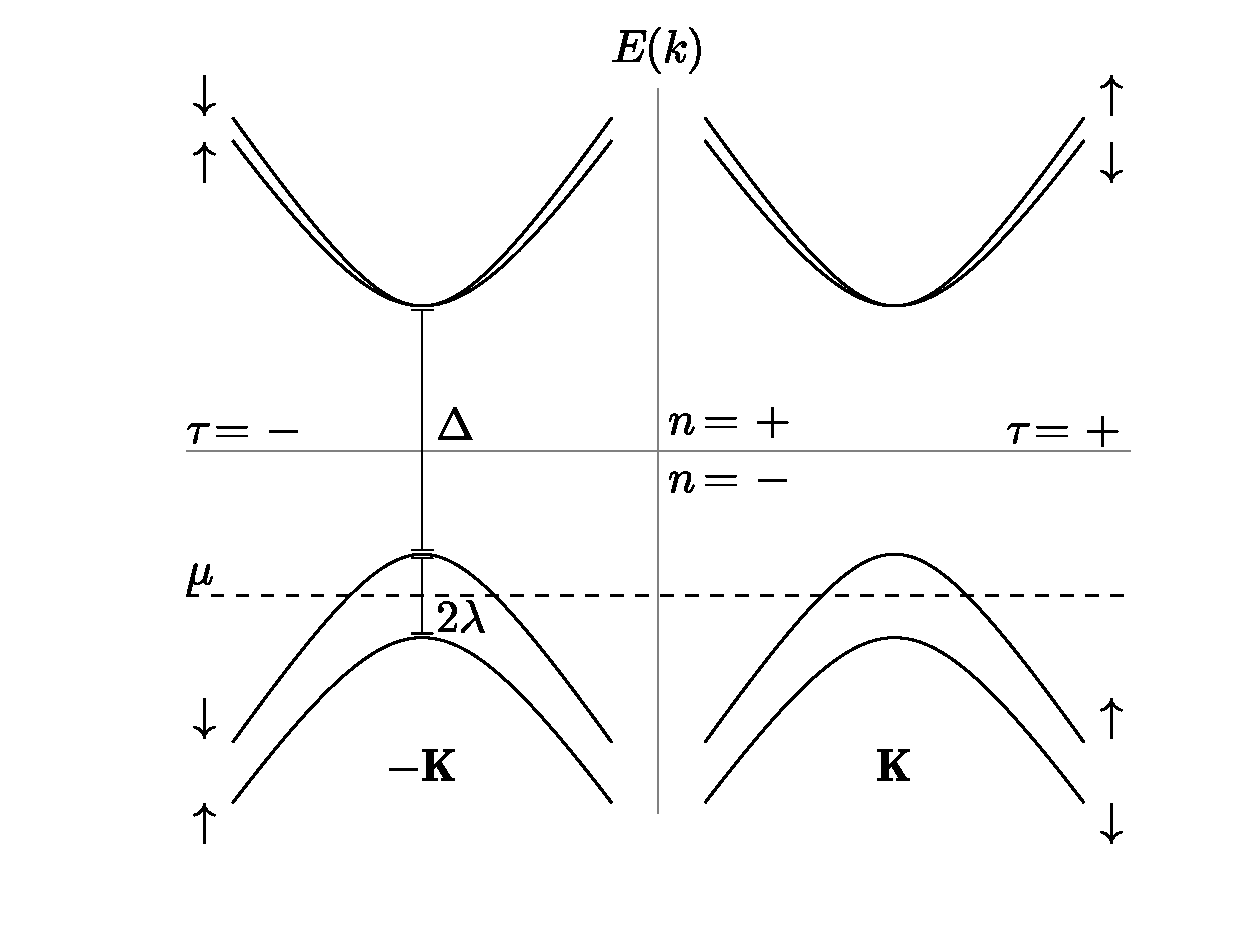
\includegraphics[width=\columnwidth]{figures/energy-bands}
  \caption{%
    Energy bands for $\ce{WSe2}$ as given by \cref{eq:energy}
    with $a t = \SI{3.939}{\electronvolt \per \angstrom}$,
    $E_g = \SI{1.60}{\electronvolt}$,
    and $E_{\text{soc}} = \SI{0.23}{\electronvolt}$.
    Each valley is centered at $± \vc{K}$ relative to the center of the
    Brillouin zone.
    The energy for a given band depends only on the distance $k$
    measured from the valley center.
  }\label{fig:energy}
\end{figure}

We focus on doped systems
such that the chemical potential $μ$ lies in the upper valence bands.
Within each band, the Bloch basis eigenstates are written
in terms of the orbital states as elements on the Block sphere,
\begin{equation}
  \begin{aligned}
    \Ket{u_{τ {\s}}^n \of{k, ϕ}}
    = & \cos{\frac{\fnTheta{n}}{2}} \ketOrb{+}{\of{k, ϕ}} \\
    + e^{-i τ ϕ}
      & \sin{\frac{\fnTheta{n}}{2}} \ketOrb{-}{\of{k, ϕ}},
  \end{aligned}
\end{equation}
where $k_x + i τ k_y = k e^{i τ ϕ}$ and
\begin{equation}
  \tan{\frac{\fnTheta{n}}{2}}
  = \frac{a t τ k}{\dfrac{E_g}{2} - \fnEnergy{-n} \of{k}}
  = \frac{a t τ k}{\fnEnergy{n} \of{k} - \fnEnergy{-} \of{0}}.
\end{equation}
The polar angle on the Bloch sphere
of the conduction and valence bands are related by
$\fnTheta{-} - \fnTheta{+} = τ π$.
The mapping of the energy band to the Bloch sphere,
parametrized by $\left( θ, ϕ \right)$,
encodes the topological character:
as one moves from the node out to infinity,
the states sweep either the northern or southern hemisphere
with a chirality determined by the Berry curvature.
